\subsection{Region transition probability}

A travel path of a taxi can be simplified as a multi-hop process, in which a hop indicates an on/off event happened. Seeing that, we define a\emph{ region transition probability} to figure out the probability of the next hop falling in a definite region $j$ from the current region $i$. Particularly, two successive events are different. Likewise, the region $i$ and $j$ are recognized by different metrics, that is, off or on event distribution. It is more reasonable. For an instance, if the taxi is occupied, the next hop event is the off one. Hence, choosing a target region from a region set divided by off event distribution is more logical.
%%ÿ���ֲ���ͷһ��Ҫ��&���ţ�����\qquad Ϊ��ո�����

To calculate the region transition probability, the \textbf{region recognition process} should be executed in advance.

Firstly, we divide the area into $100\times 100$ grids, and define cells in it as equation \ref{cell}. Then, we consider region as adjacent cells as equation \ref{region}. 

\begin{equation}\label{cell}
\begin{array}{c}
CELL_{x,y}::=\{(lon,lat)|x \le \frac{{lon}}{{len_x}} < x + 1,\\
y \le \frac{{lat}}{{len_y}} < y + 1\}
\end{array}
\end{equation}

\begin{equation}\label{region}
  \begin{array}{r}
REGION_m:: = \{ CEL{L_{x,y}}|\exists CELL_{i,j} \in REGION_m\\
\Rightarrow \|x - i\| \le 1,\|y - j\| \le 1\}
\end{array}
\end{equation}

By clustering cells into regions, two set of region $\{REGION_m^{on}\}$ and $\{REGION_n^{off}\}$ can be recognized. The clustering idea is to put adjacent cells with event density larger than the event threshold $\eta$ into one cluster. To avoid the size of the region become too large or too small, we set a $CLUSTERSIZE$ to restrict a region, say $\|REGION_i\|\leq CLUSTERSIZE$ , and only limit the top 200 regions, in which $CELL_{x,y}.events\geq \eta$. After that, the other cells not belong to the top 200 regions, will be cluster into regions, while $\|REGION_j\|\leq CLUSTERSIZE$. 
We sort the cells by event density in descending order, and begin with the first cell to search is neighbors whether to join the same region using breadth traversal. The region recognition results for on/off events are shown in figure \ref{figure_region_recognizition}. The detail clustering algorithm is presented in the appendix. In addition, the $CLUSTERSIZE=200$, $\eta=121$ for on event and $\eta=141$ for off event set by the average event density of the top 5000 cells order by its event density.

\begin{figure}[htbp]
\centering
\subfigure[passenger off event regions]{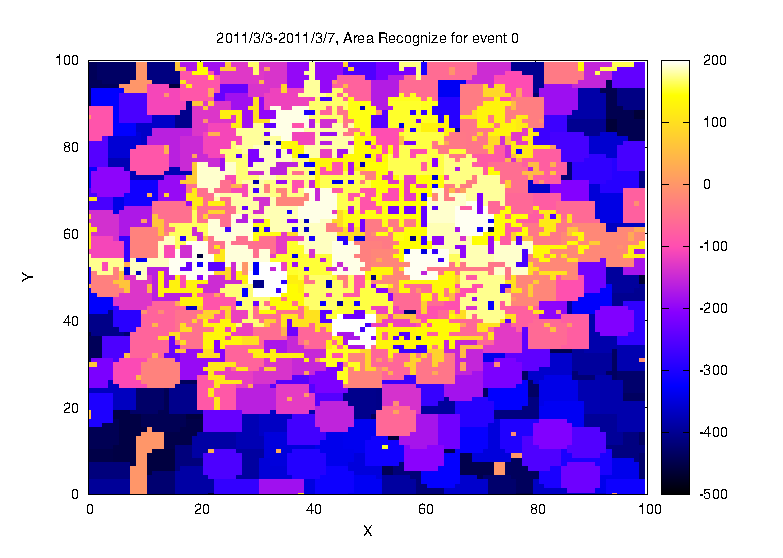
\includegraphics[width=0.4\textwidth]{figures_201103/region/Areas-2011_event0.eps}}
\subfigure[passenger on event regions]{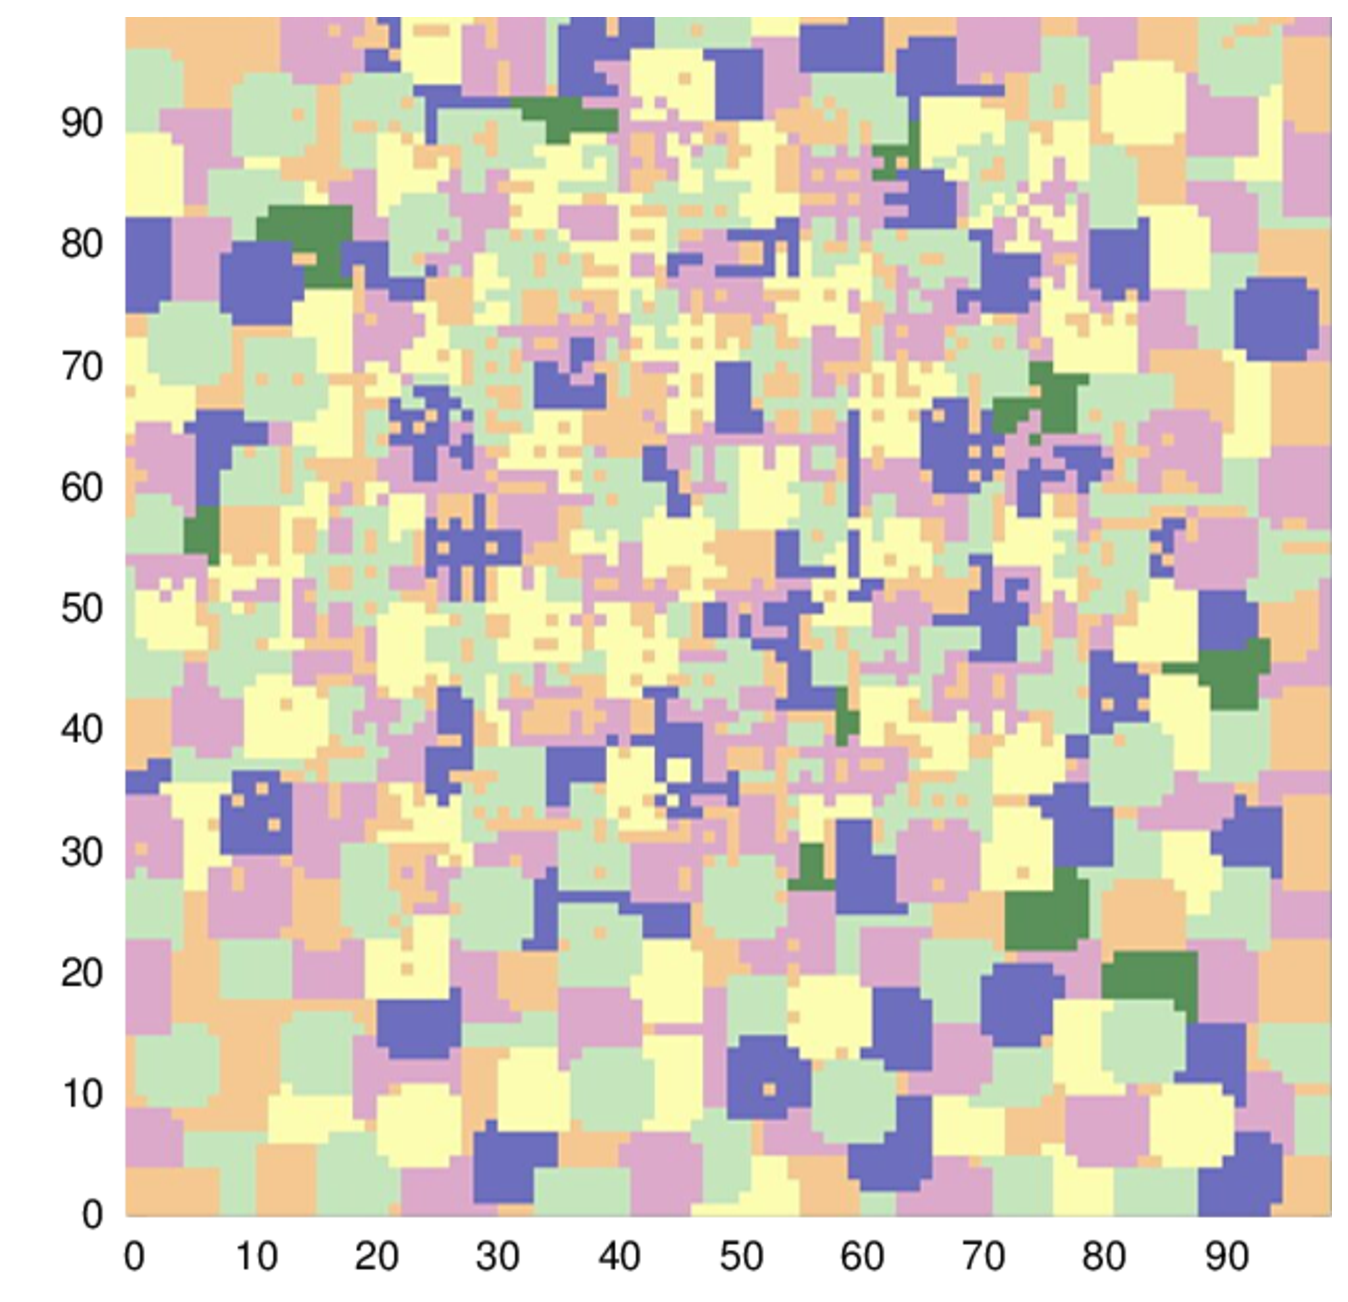
\includegraphics[width=0.4\textwidth]{figures_201103/region/Areas-2011_event1.eps}}
\centering
\caption{Region recognition}\label{figure_region_recognizition}
\end{figure}

\textbf{The calculate process of the region transition probability:} After clustering cells into regions, the transition probability from $REGION_i^{on/off}$ to $REGION_j^{off/on}$, donated as $p_{i\rightarrow j}^{on\rightarrow off /off\rightarrow on}$. To substantiate, the calculate process of $p_{i\rightarrow j}^{on\rightarrow off}$ will be introduced in detail. Clearly, the records of $event=on$ in $REGION_i^{on}$ can be required from the data set. the record amount is donated as $\|RECORDS_i^{on}=\{record_{REGION_i^{on}}\}\|$. For $record \in RECORD_i^{on}$, the next event and location can be easily required. Therefore, the record can be associated with the its next hop information to $(taxiid, location_{current}, event,event_{next},location_{next})$. The $RECORDS_{i\to j}^{on\to off}=\{record|event=on\cap event_{next}=off\cap location_{current}\in REGION_i^{on}\cap location_{next}\in REGION_j^{off}\}$ will be obtain.

\begin{equation}\label{pij}
p_{i \to j}^{on \to off} = \frac{\|RECORDS_{i\to j}^{on\to off}\|}{\|RECORDS_i^{on}\|}
\end{equation}


\begin{equation}\label{transition_matrix}
  P^{on\to off} = (p_{i\to j}^{on\to off})_{m*n}  
\end{equation}

\begin{equation}\label{transition_matrix}
  P^{off\to on} = (p_{i\to j}^{off\to on})_{n*m}
\end{equation}

%%\begin{equation}\label{equation_taxiset_matrix}
%\textbf{\emph{P^{on\to off}}}=(p_{i\to j}^{on\to off})_{m*n}\\
%\textbf{\emph{P^{off\to on}}}=(p_{i\to j}^{off\to on})_{n*m}\\
%\end{equation}

